\section{Introdução}


\begin{frame}
  \frametitle{\emph{Main Achievement} deste trabalho}

    Desenvolvimento de uma técnica para \alert{monitorar a posição de qualquer objeto no espaço usando RF-ID}.

    \begin{itemize}
      \item Com \alert{alta precisão} (erro de 3.5 cm)
      \item Em \alert{tempo real}
      \item Funciona mesmo em ambientes \alert{indoor}
    \end{itemize}
\end{frame}

\section{E para que serve isso?}

\begin{frame}
  \begin{center}
    \Huge E para que serve isso?
  \end{center}
\end{frame}

\begin{frame}
  \frametitle{Interação homem-máquina}
  \begin{figure}
    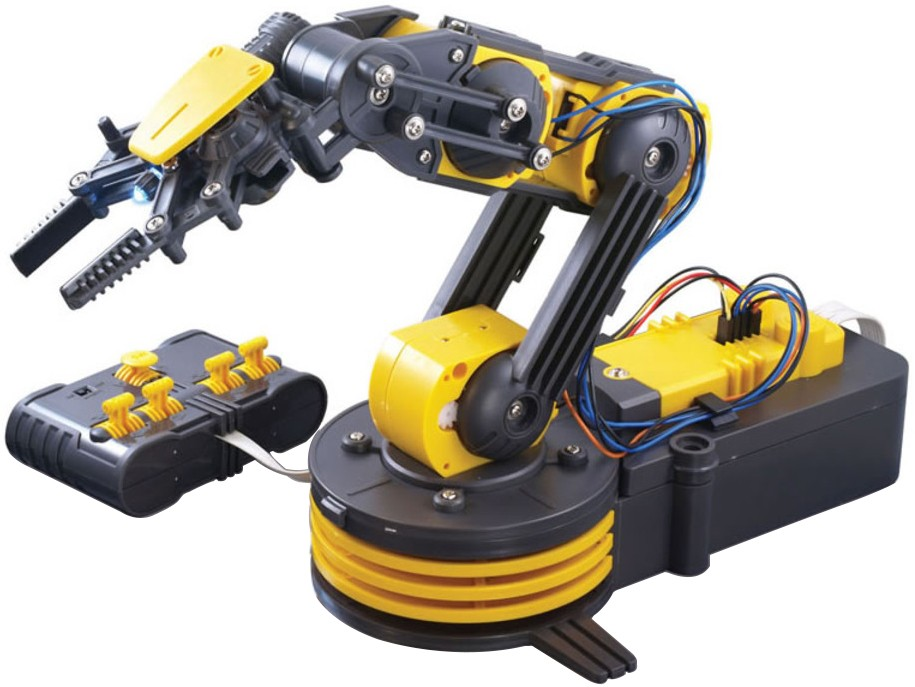
\includegraphics[width=.8\textwidth]{robot-arm}
		\caption*{Controle / monitoração de braços robóticos}
  \end{figure}
\end{frame}

\begin{frame}
  \frametitle{Interação homem-máquina}
  \begin{figure}
    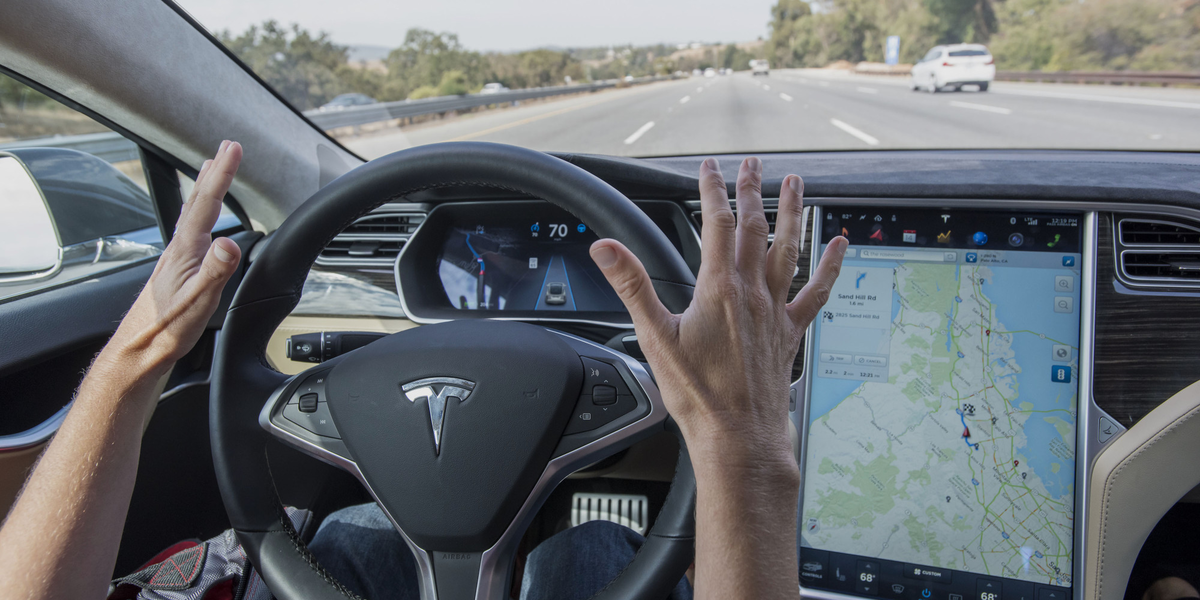
\includegraphics[width=\textwidth]{autopilot}
		\caption*{\emph{Environment-sensing} em carros autônomos}
  \end{figure}
\end{frame}

\begin{frame}
  \frametitle{Jogos / Realidade aumentada}
    \begin{columns}[T,onlytextwidth]
        \column{.5\textwidth}
					\begin{figure}
							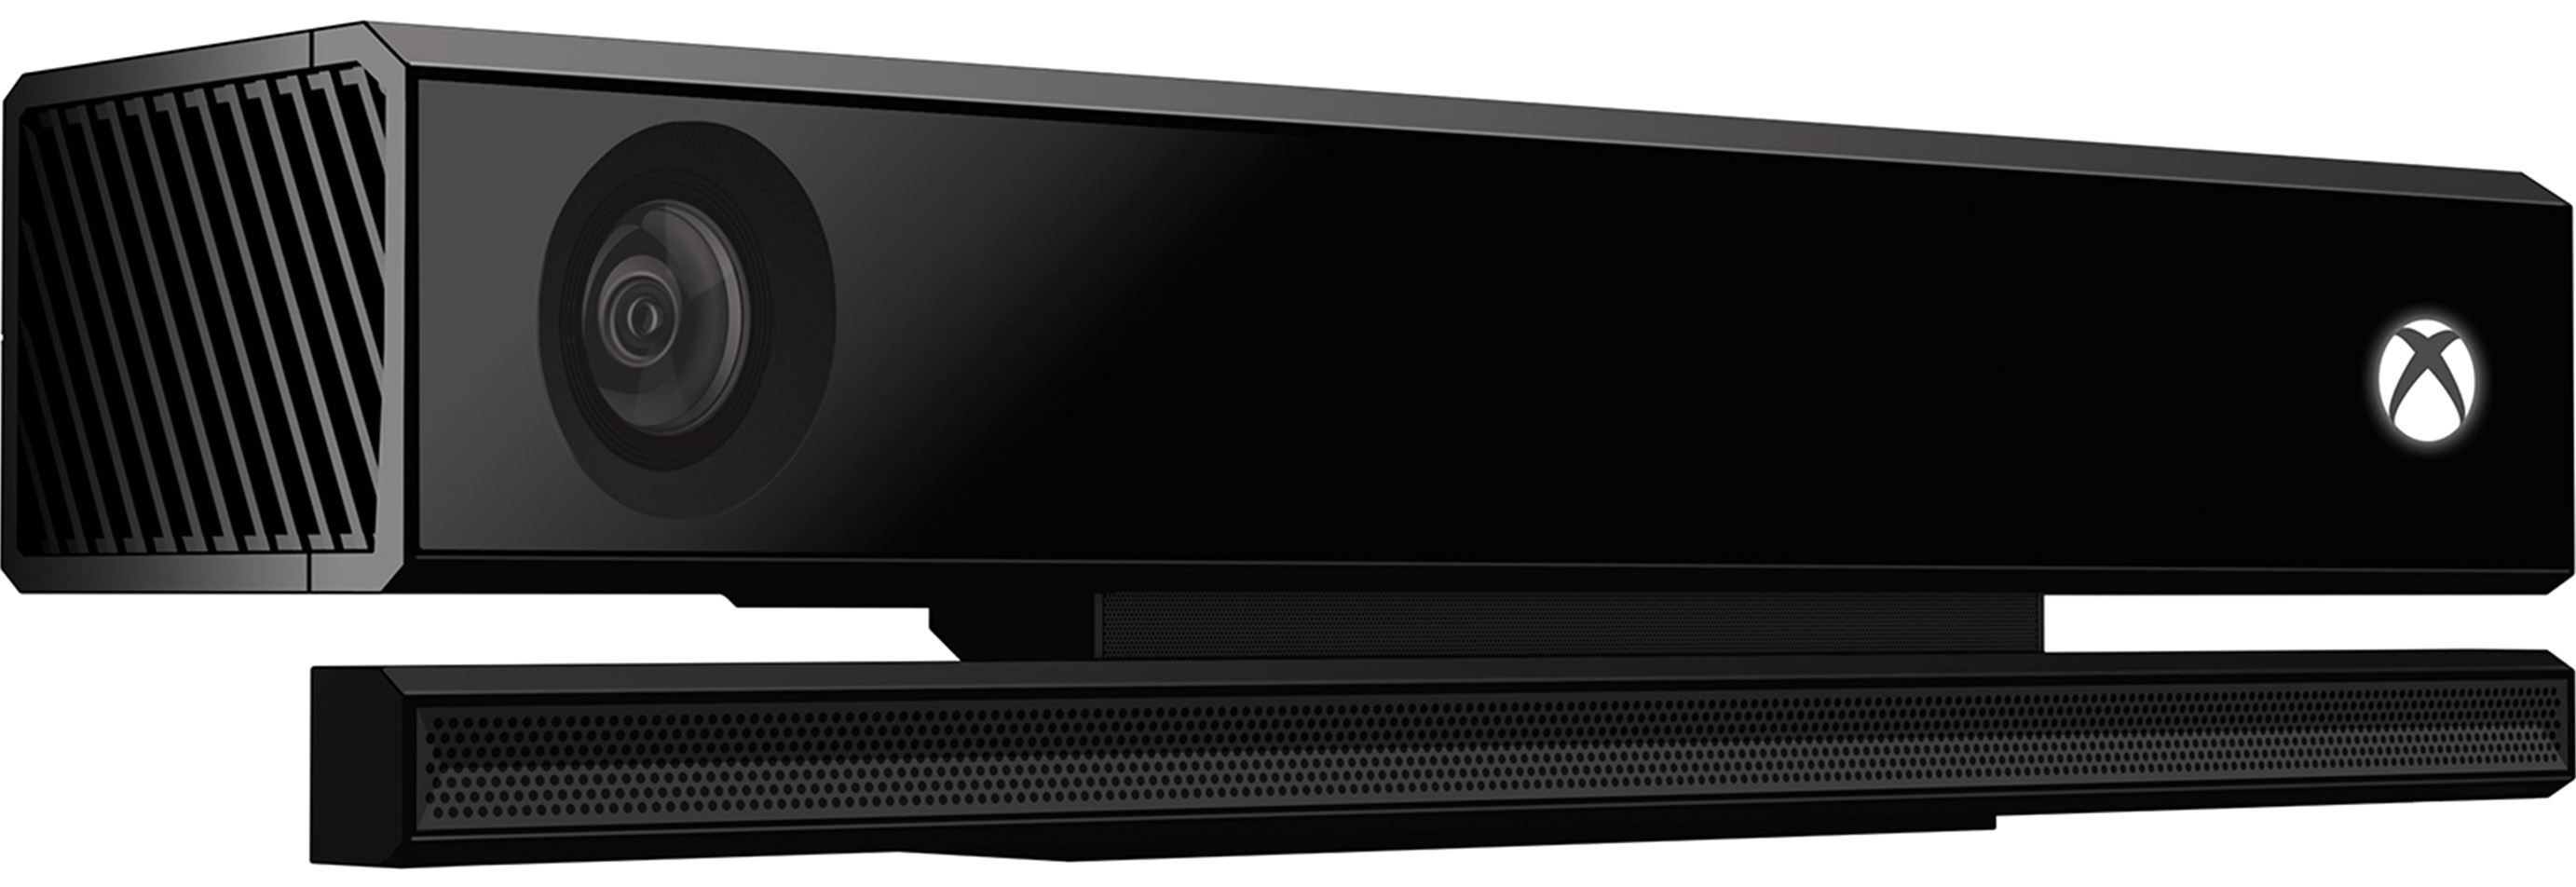
\includegraphics[width=\textwidth]{kinect}
						\captionsetup{labelformat=empty}
						\caption{Kinect motion sensor}
					\end{figure}

        \column{.5\textwidth}
					\begin{figure}
							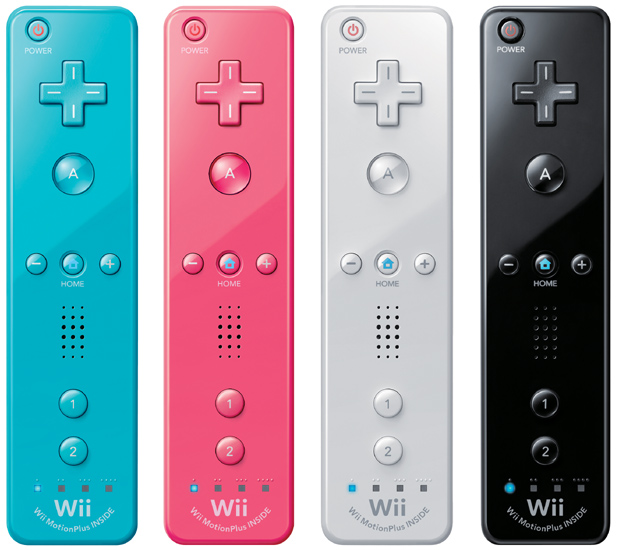
\includegraphics[width=0.5\textwidth]{wii-controller-more}
						\captionsetup{labelformat=empty}
						\caption{Controles Wii}
					\end{figure}
    \end{columns}
\end{frame}

\begin{frame}
  \frametitle{Aplicações comerciais}
    %\begin{columns}[T,onlytextwidth]
        %\column{.5\textwidth}
					\begin{figure}
							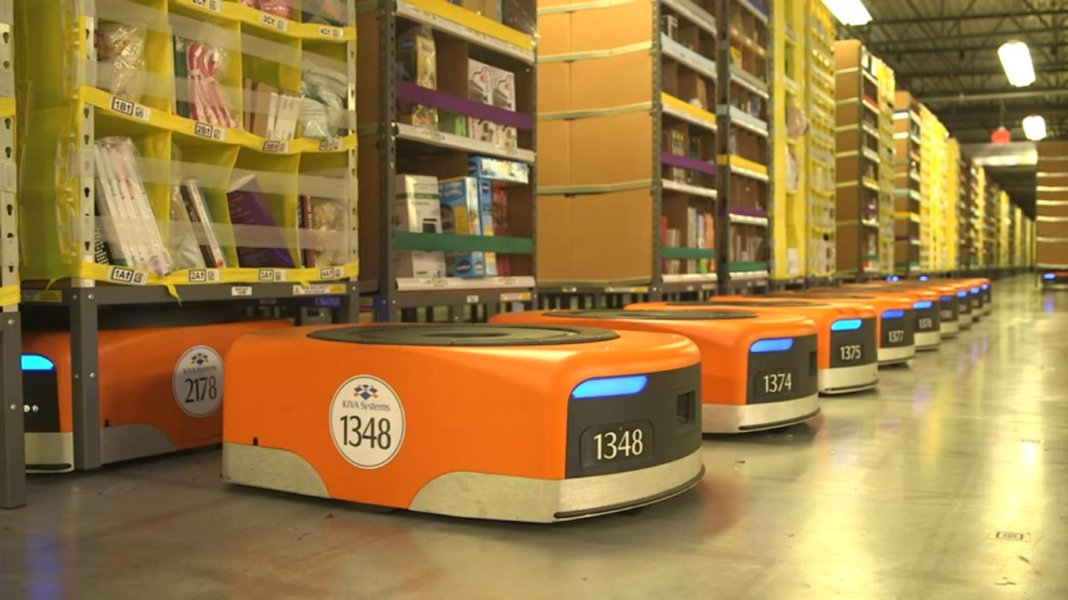
\includegraphics[width=\textwidth]{amazon-robots}
						\captionsetup{labelformat=empty}
						\caption{Robôs de distribuição Amazon}
					\end{figure}
    %\end{columns}
\end{frame}

\begin{frame}
  \frametitle{Aplicações comerciais}
    %\begin{columns}[T,onlytextwidth]
        %\column{.5\textwidth}
					\begin{figure}
							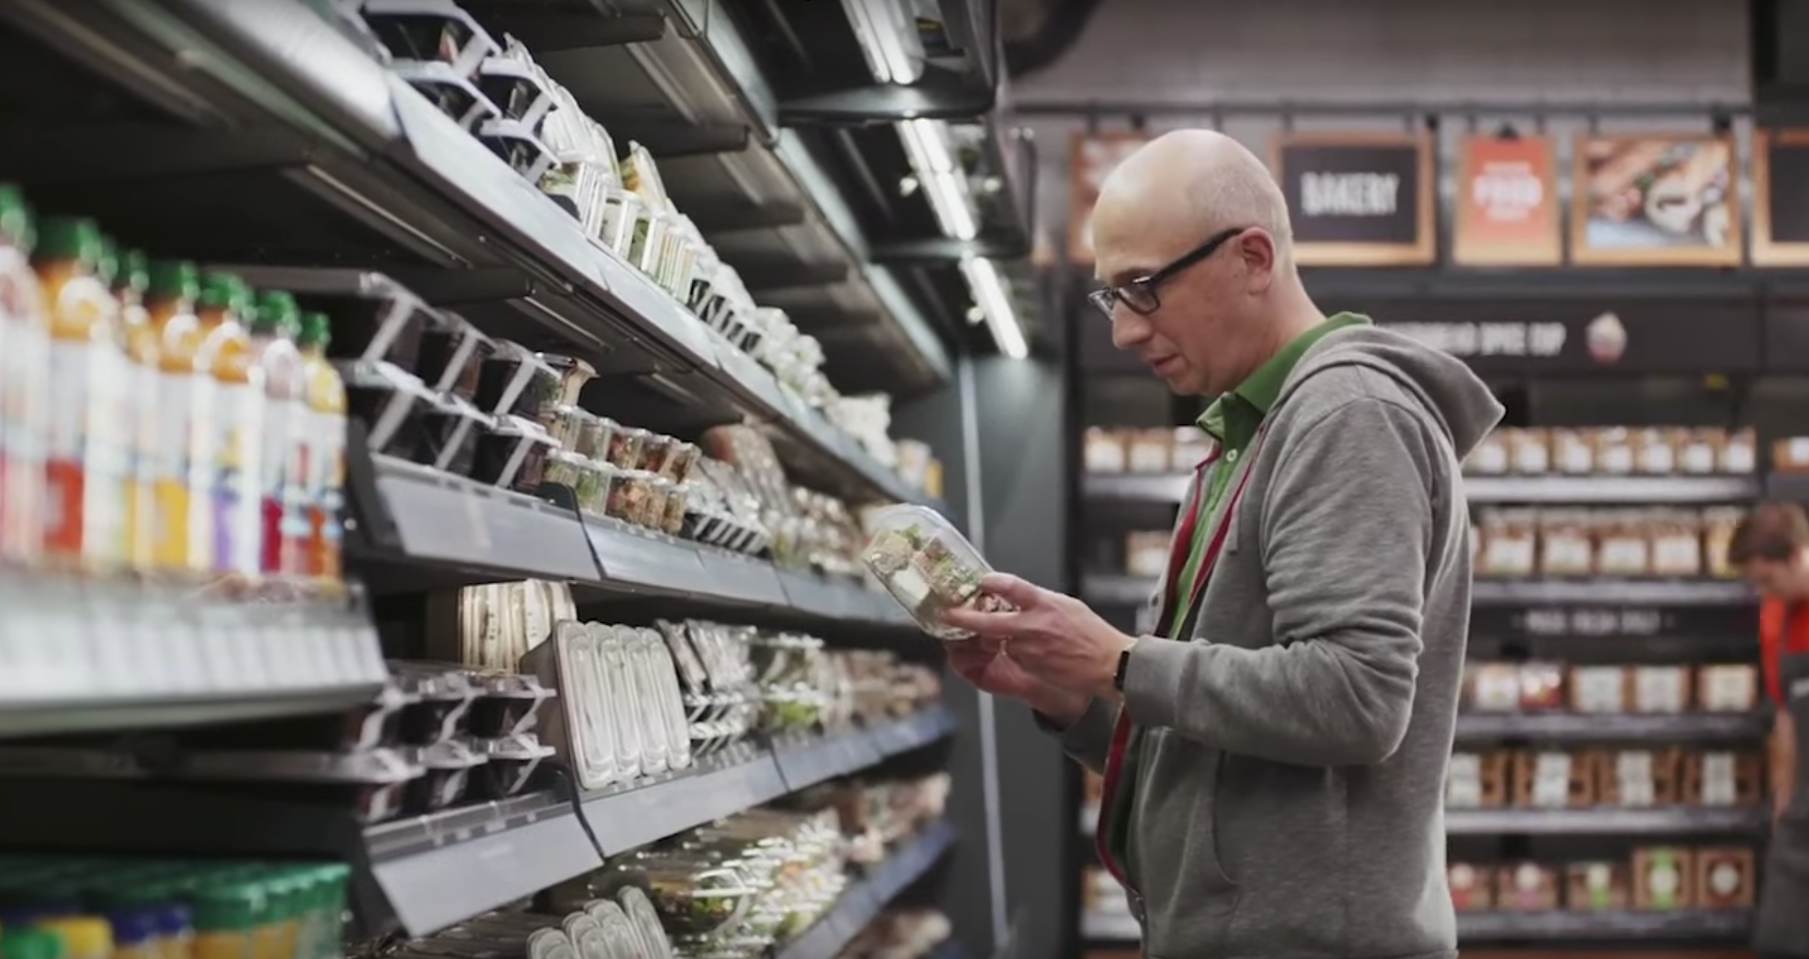
\includegraphics[width=\textwidth]{amazon-go-customer}
						\captionsetup{labelformat=empty}
						\caption{Amazon Go}
					\end{figure}
    %\end{columns}
\end{frame}

\begin{frame}
  \frametitle{3D-Tracking hoje}

  Boa parte das técnicas de 3D-Tracking atuais são baseadas em visão computacional, com pequenas variações:
  \begin{itemize}
    \item no número de câmeras utilizadas
    \item nos algoritmos de CV utilizados
    \item etc
  \end{itemize}
\end{frame}

\begin{frame}
  \frametitle{O problema já não está então resolvido?}

  Limitações das soluções atuais
  \begin{itemize}
    \item  Alta complexidade computacional
    \item  Custo de implementação
    \item  Não funcionam em ambientes com obstáculos
  \end{itemize}

	\begin{figure}
			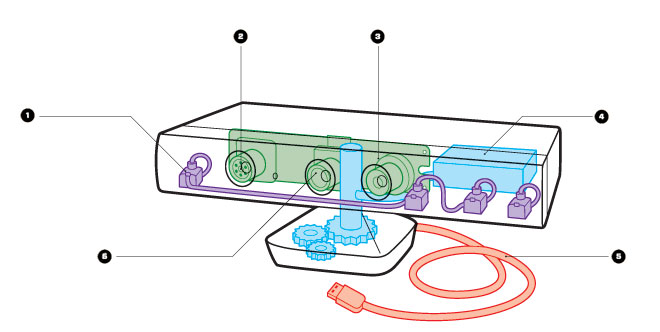
\includegraphics[width=0.8\textwidth]{kinect-diagram}
		\captionsetup{labelformat=empty}
		\caption{Diagrama de um Kinect}
	\end{figure}
\end{frame}


\begin{frame}
  \frametitle{3D-Tracking com RF-ID}

  Vantagens
  \begin{itemize}
    \item  \alert{Tags são muito baratas} ($0.1 \sim 0.2$ dólares)!
    \item  Técnica \alert{funciona mesmo com obstáculos}
    \item  \alert{Menor complexidade computacional}!
  \end{itemize}

  Problemas do estado-da-arte que a técnica que apresentaremos supera
  \begin{itemize}
    \item  Dependência de antenas de referência ou \emph{anchor nodes} 
    \item  Dependência de conhecimento prévio da trajetória
    \item  Limitação a 2D-Tracking
  \end{itemize}
\end{frame}
